\documentclass[12pt, a4paper]{article}
\usepackage[francais]{babel}
\usepackage{caption}
\usepackage{graphicx}
\usepackage[T1]{fontenc}
\usepackage{listings}
\usepackage{geometry}
\usepackage{amsmath}
\usepackage{listings}
\usepackage[colorlinks=true,linkcolor=black,anchorcolor=black,citecolor=black,filecolor=black,menucolor=black,runcolor=black,urlcolor=black]{hyperref}

% \usepackage{mathpazo} --> Police à utiliser lors de rapports plus sérieux

\usepackage{fancyhdr}
\pagestyle{fancy}
\lhead{}
\rhead{}
\chead{}
\rfoot{\thepage}
\lfoot{Martin Baumgaertner}
\cfoot{}

\renewcommand{\headrulewidth}{0.4pt}
\renewcommand{\footrulewidth}{0.4pt}

\begin{document}
\begin{titlepage}
	\newcommand{\HRule}{\rule{\linewidth}{0.5mm}} 
	\center 
	\textsc{\LARGE iut de colmar}\\[6.5cm] 
	\textsc{\Large R405 Automatisation des tâches}\\[0.5cm] 
	\textsc{\large Année 2022-23}\\[0.5cm]
	\HRule\\[0.75cm]
	{\huge\bfseries TP 3 : PING}\\[0.4cm]
	\HRule\\[1.5cm]
	\textsc{\large martin baumgaertner}\\[6.5cm] 

	\vfill\vfill\vfill
	{\large\today} 
	\vfill
\end{titlepage}
\newpage
\tableofcontents
\newpage
\section{Introduction}
Ce premier TP a pour objectif de vous faire manipuler le programme ping sous 
Bash. Vous utiliserez pour cela, une machine virtuelle Linux. Durant ce TP 
vous devrez produire un compte rendu au format PDF qui contient les commandes 
et scripts Bahs associés aux questions accompagnés d’une explication. La 
première page du rapport devra contenir votre nom et prénom ainsi que le 
numéro du TP réalisé. Ces comptes rendus seront relevés et devront être 
déposés sur Moodle, les noms des comptes rendus devront être de la forme 
TP1-Bash-Nom- Prénom. Vous utiliserez la commande ping en respectant cet 
ordre pour les paramètres : ping [option] adresseIP et vous n’utilisez pas 
l’option –w (en raison de l’implémentation bash sous MAC).

\section{Exercice 1}

Voici donc le script que j'ai trouvé. Premièrement on demande à l'utilisateur de rentrer
l'adresse IP qu'il veut tester en boucle. Puis on vient la tester comme demandé dans l'énoncé.
\begin{figure}[h]
    \centering
    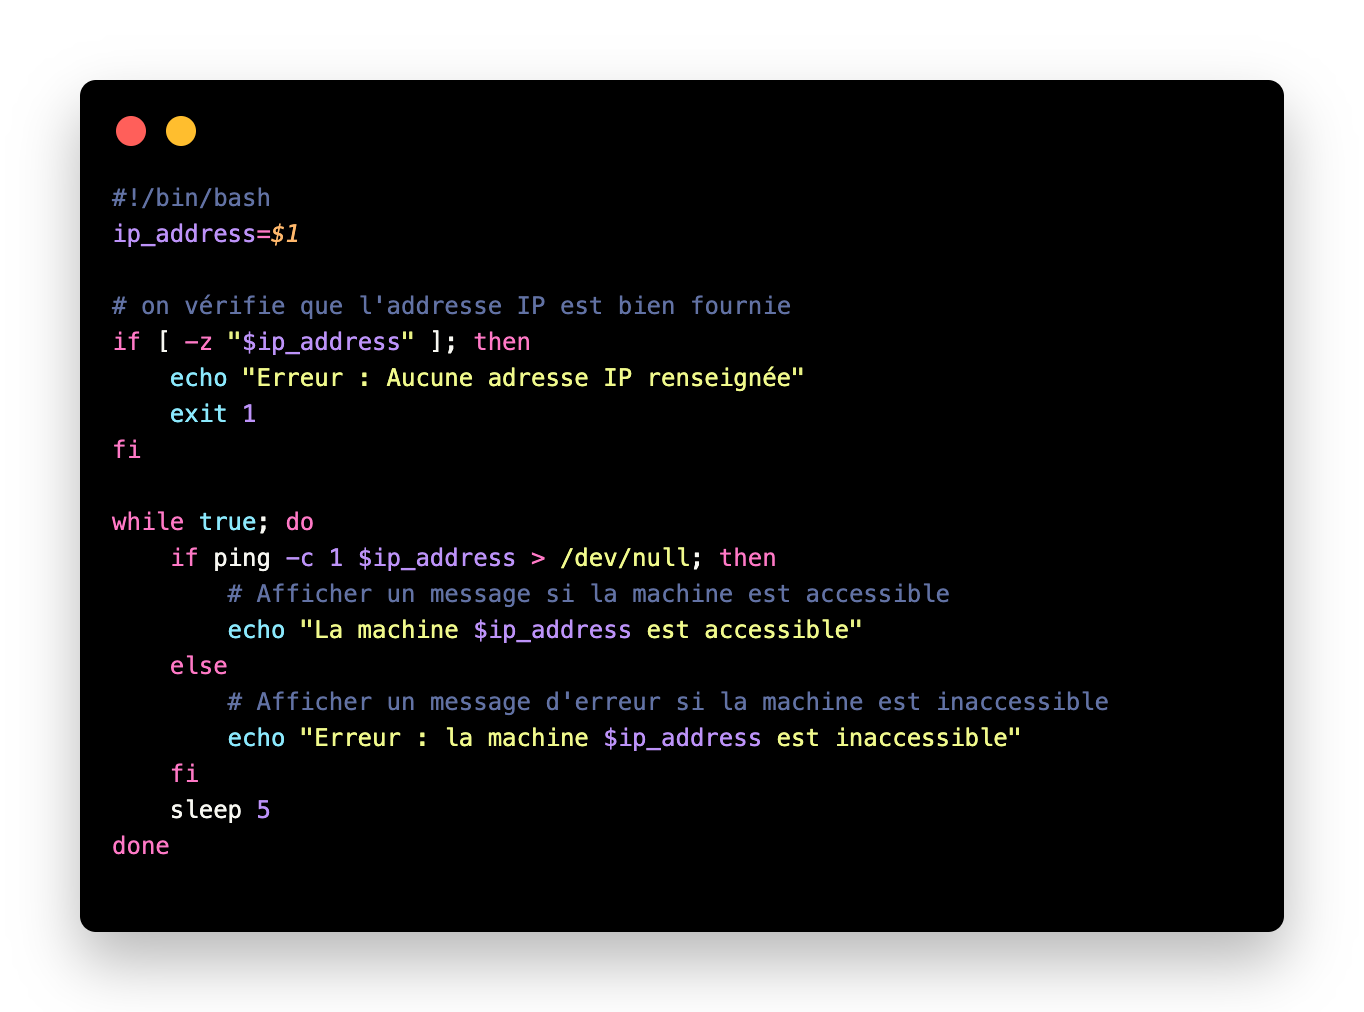
\includegraphics[width=0.9\textwidth]{img/code1.png}
    \caption{Premier script}
    \label{fig:script1}
\end{figure}\\

Voici les droits sur mon script pour vous prouver qu'il n'a pas été réalisé en 
\textbf{root} :
\begin{figure}[h]
    \centering
    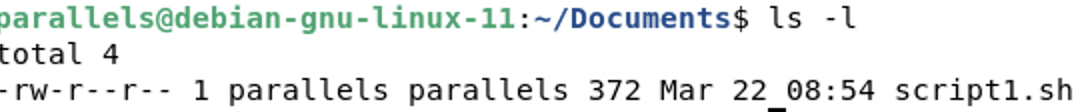
\includegraphics[width=1\textwidth]{img/preuve1.png}
    \caption{Preuve droits script}
    \label{fig:script2}
\end{figure}\\
Comme le démontre la capture d'écran, le script à été réalisé en tant que utilisateur
\textbf{parallels}. Cet utilisateur correspond à l'utilisateur par défaut des machines
virtuelles virtualisés par \textbf{parallels desktop}, logiciel de virtualisation sur MacOS.

\newpage
\section{Exercice 2}
Voici donc le script que j'ai crée. J'ai juste repris le code précédent et 
ajouté l'enregistrement des résultats dans un fichier texte. 
\begin{figure}[h]
    \centering
    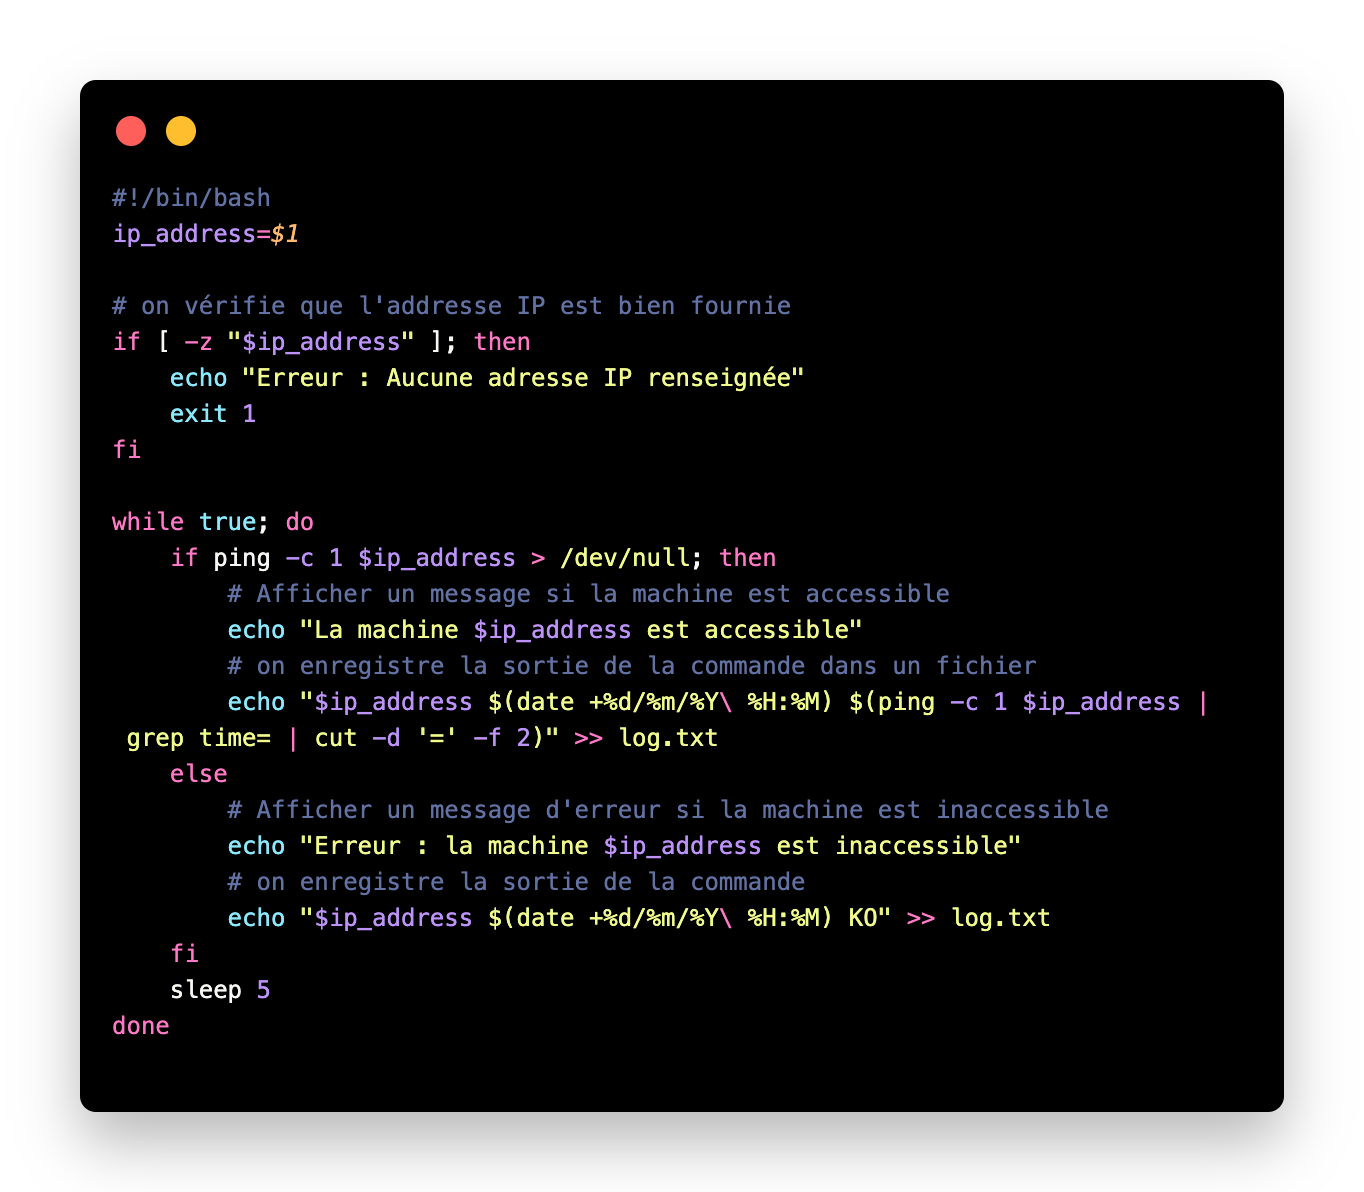
\includegraphics[width=0.8\textwidth]{img/code2.png}
    \caption{Deuxième script}
    \label{fig:script3}
\end{figure}\\
Comme avant, voici les droits sur le fichier : 
\begin{figure}[h]
    \centering
    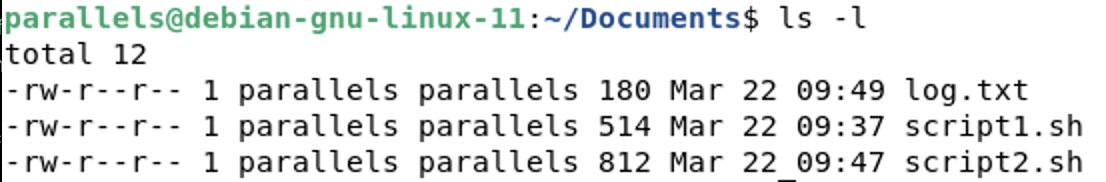
\includegraphics[width=1\textwidth]{img/preuve2.png}
    \caption{Preuve droits script}
    \label{fig:script4}
\end{figure}\\
\newpage
Et voici ce que l'on obtient dans le fichier de log, on a bien 
le format qu'il était demandé : 
\begin{figure}[h]
    \centering
    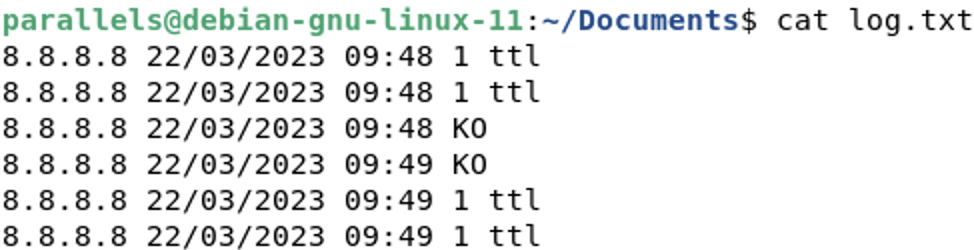
\includegraphics[width=1\textwidth]{img/log.png}
    \caption{Fichier logs}
    \label{fig:script5}
\end{figure}\\
\section{Exercice 3}
Vous pouvez donc voir à la page suivante le troisième script que j'ai réalisé.
Nous pouvons tout d'abord voir que j'ai crée un fichier avec les adresses IP à tester 
et que nous avons toujours dans le fichier de log les résultats des commandes :\\ 

\begin{figure}[h]
    \centering
    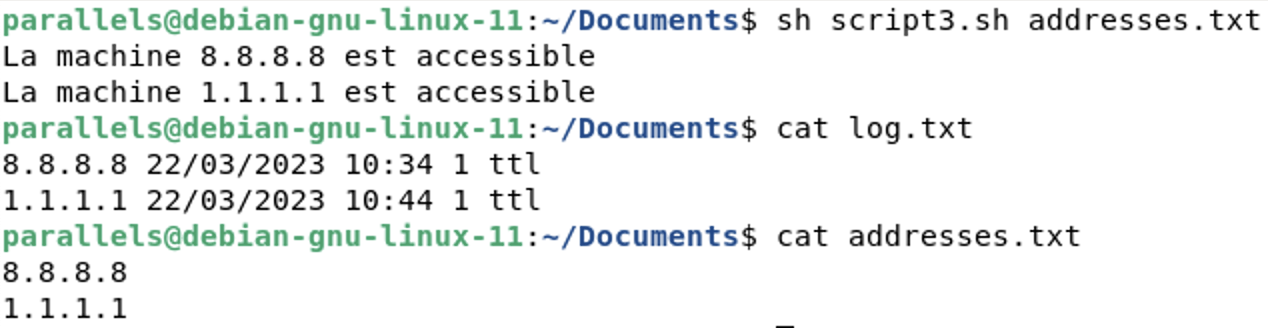
\includegraphics[width=1\textwidth]{img/preuve3.png}
    \caption{Preuve 3}
    \label{fig:script6}
\end{figure}

\begin{figure}[h]
    \centering
    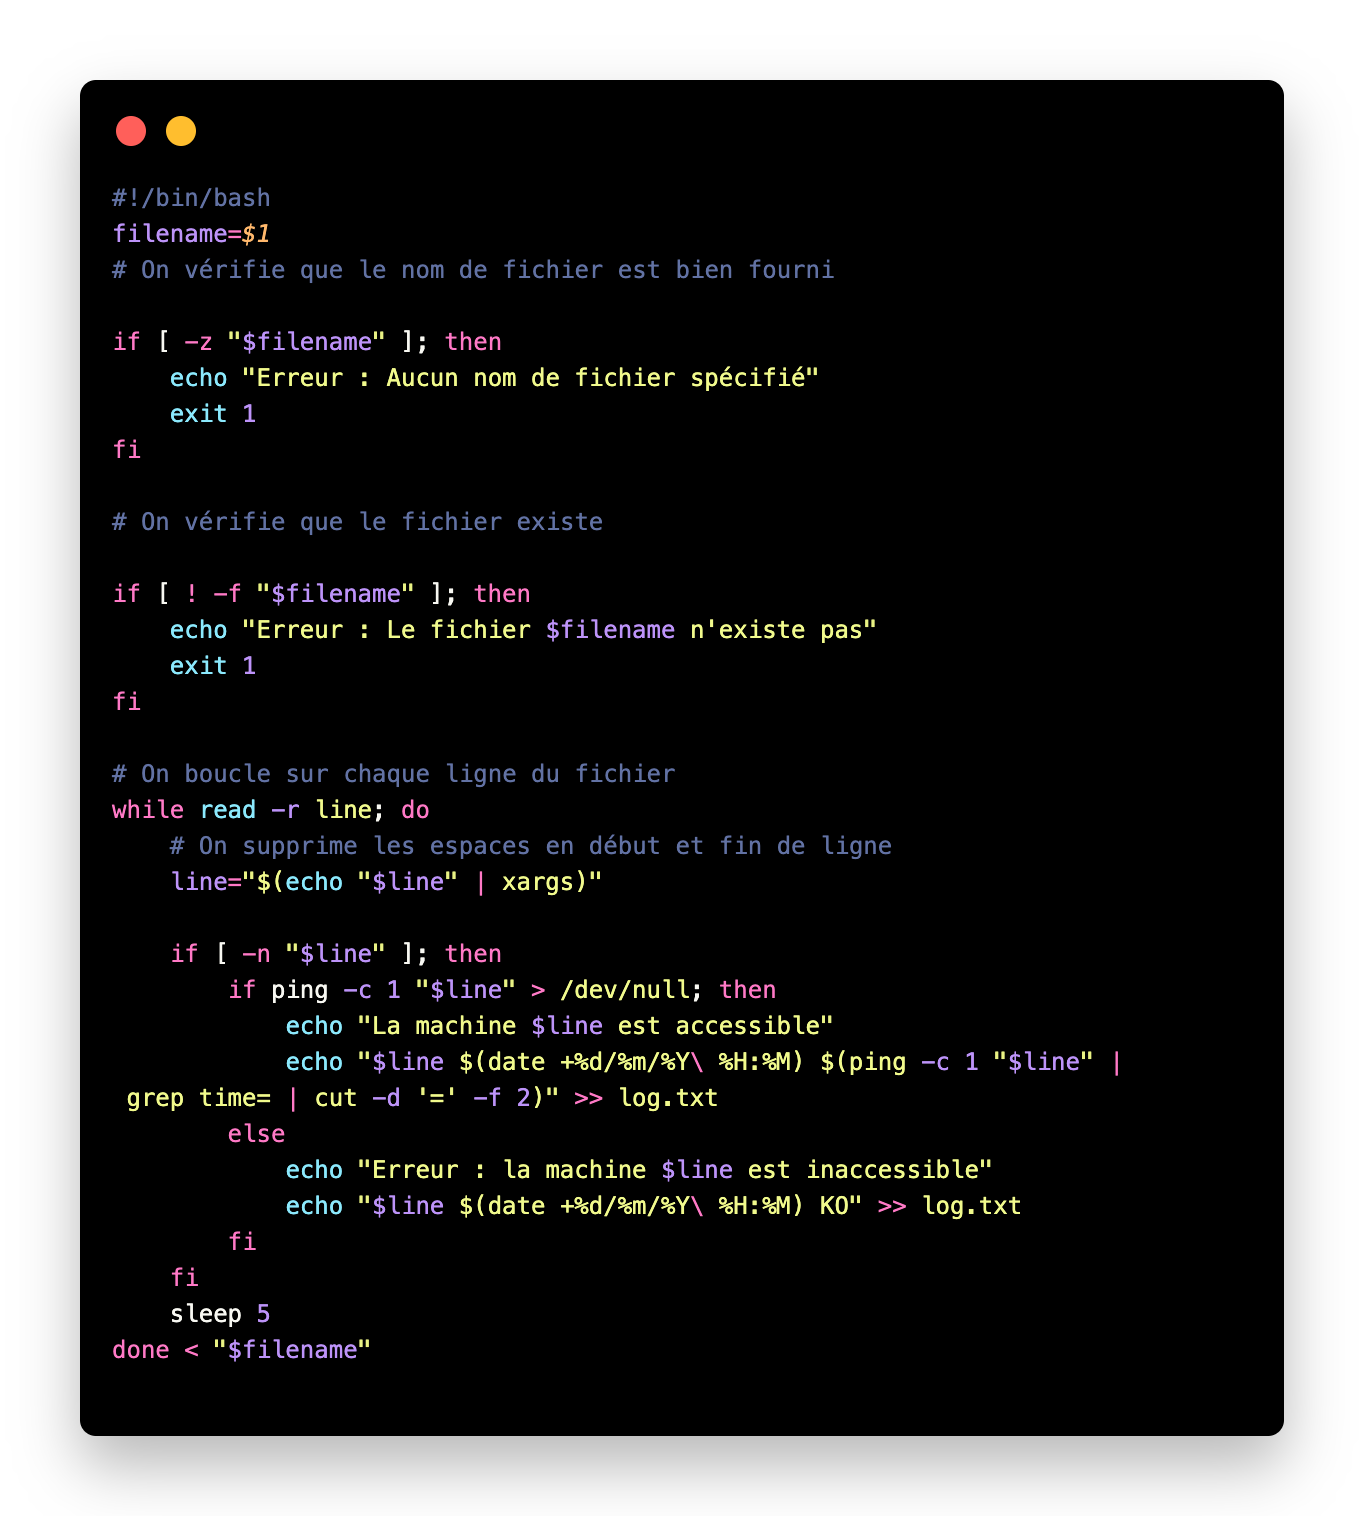
\includegraphics[width=1\textwidth]{img/code3.png}
    \caption{Troisième script}
    \label{fig:script7}
\end{figure}

\end{document}